\begin{appendix}
\addcontentsline{toc}{section}{Appendix}
\label{sec:appendix}

\section{Android Applikation - Screenshots}

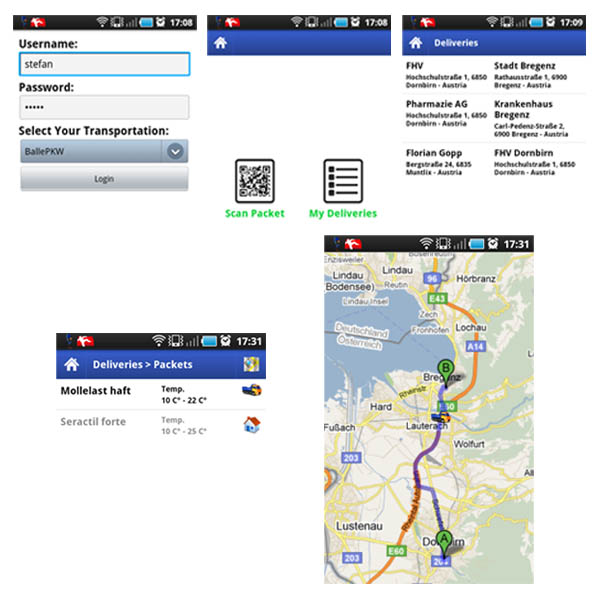
\includegraphics[width=140mm]{files/AndroidApp.jpg}

\section{Kommerzielle Temperatursensoren}
	\paragraph{Hygrosens TLOG20-BLUE}
		Das ist \textit{NICHT} unsere Lösung.
		\url{http://shop.hygrosens.com/Messsysteme-acma/
			Messsysteme-fuer-Temperatur/Temperaturmesssysteme/
			Temperaturmesssysteme-BLUETOOTH/
			BLUETOOTH-Temperaturmesssystem-20-Kanaele.html}
			{hygrosens.com/TLOG20-BLUE, Zugriff am 16.04.2011}
	\par
	
	\paragraph{Ampedrf BT11}
		Das ist \textit{NICHT} unsere Lösung.
		\url{http://www.ampedrf.com/modules.htm}
		{BT11 Class1, Zugriff am 16.04.2011}
		\url{http://www.ampedrf.com/datasheets/BT11_Datasheet.pdf}
		{BT11 Datasheet}
	\par 

	\paragraph{\$149 Programmable Universal Key Fob Sensor}
		Wir haben uns für das BlueRadios BR-FOB-SEN-LE4.0 Device  entschieden, weil es
		eine komplette und etablierte Lösung für Temperatur, Beschleunigungs- und
		Licht-Messung ist.
		\url{http://www.blueradios.com/BR-FOB-SEN-LE4.0-S2A.pdf}
		{Blueradios BR-FOB-SEN-LE4, Zugriff am 16.04.2011}
		
		\url{http://www.blueradios.com/hardware_sensors.htm}
		{Blueradios BR-FOB-SEN-LE4}
	\par
	
\end{appendix}
